\subsection{题目描述}
\noindent
Consider the Poisson equation:
\[
    \nabla^2 \varphi(x, y) = -\frac{\rho(x, y)}{\varepsilon_0}
\]
from electrostatics on a rectangular geometry with \(x \in [0, L_x]\) and \(y \in [0, L_y]\). Write a program that solves this equation using the relaxation method and test your program with the following cases:

\noindent
(a) \(\rho(x, y) = 0\), \(\varphi(0, y) = \varphi(L_x, y) = \varphi(x, 0) = 0\), \(\varphi(x, L_y) = 1 \, \text{V}\),
\(L_x = 1 \, \text{m}\), and \(L_y = 1.5 \, \text{m}\);

\noindent
(b) \(\frac{\rho(x, y)}{\varepsilon_0} = 1 \, \text{V/m}^2\), \(\varphi(0, y) = \varphi(L_x, y) = \varphi(x, 0) = \varphi(x, L_y) = 0\), and \(L_x = L_y = 1 \, \text{m}\).


\subsection{程序描述}

\subsection{伪代码}
Powered by \href{https://chatgpt.com/g/g-xJJAA2awf-latex-pseudocode-generator}{\LaTeX \ pseudocode generator}


\subsection{结果示例}
\subsubsection{Case (a):无源电荷,三边接地}
\begin{figure}[H]
    \centering
    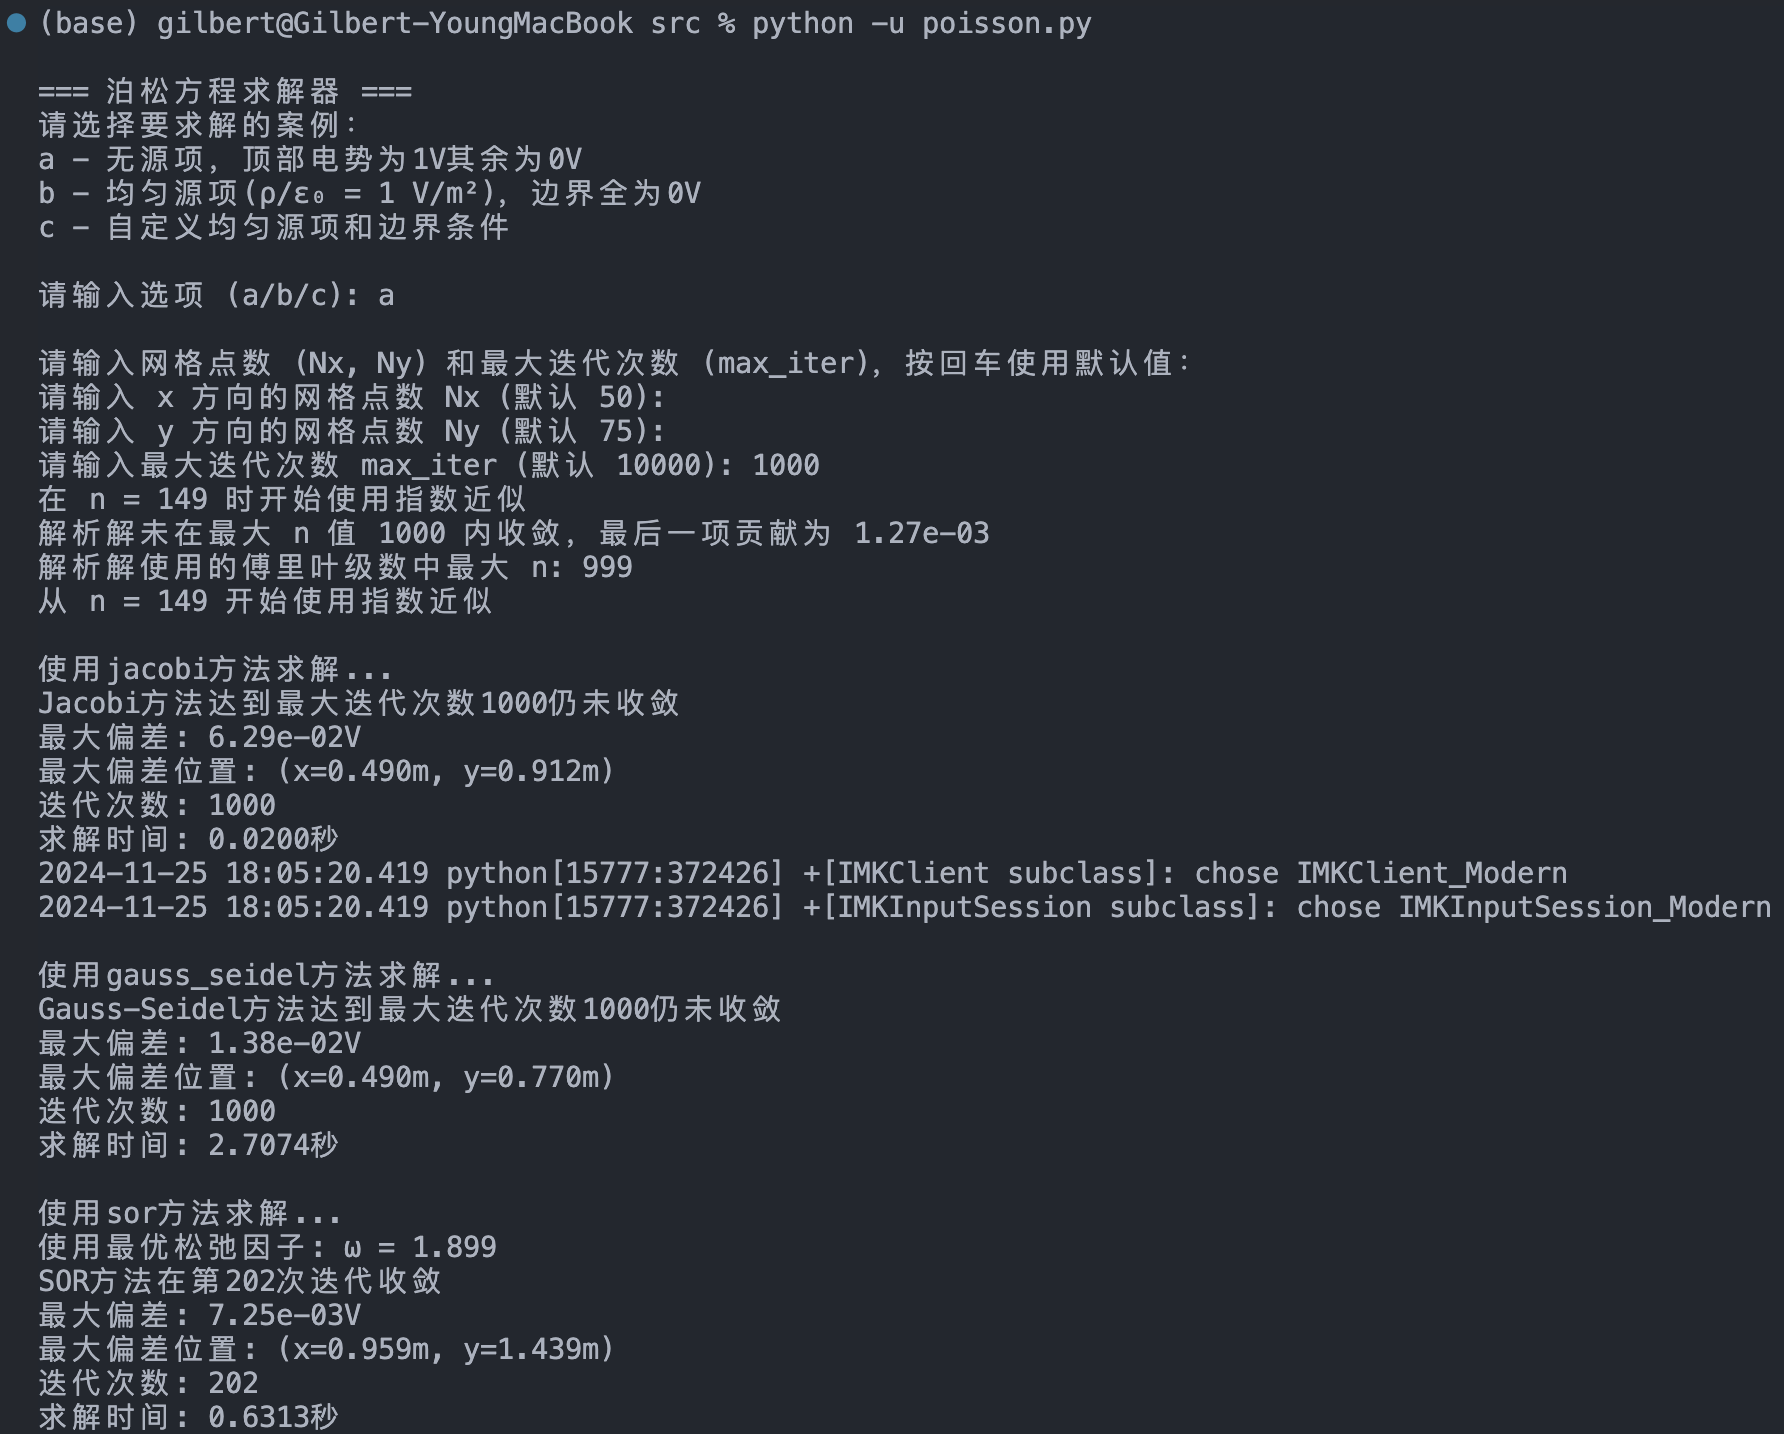
\includegraphics[width=1.0\textwidth]{Problem_1/figs/a_terminal.png}
    \caption{(a):终端输出}
\end{figure}

\begin{figure}[H]
    \centering
    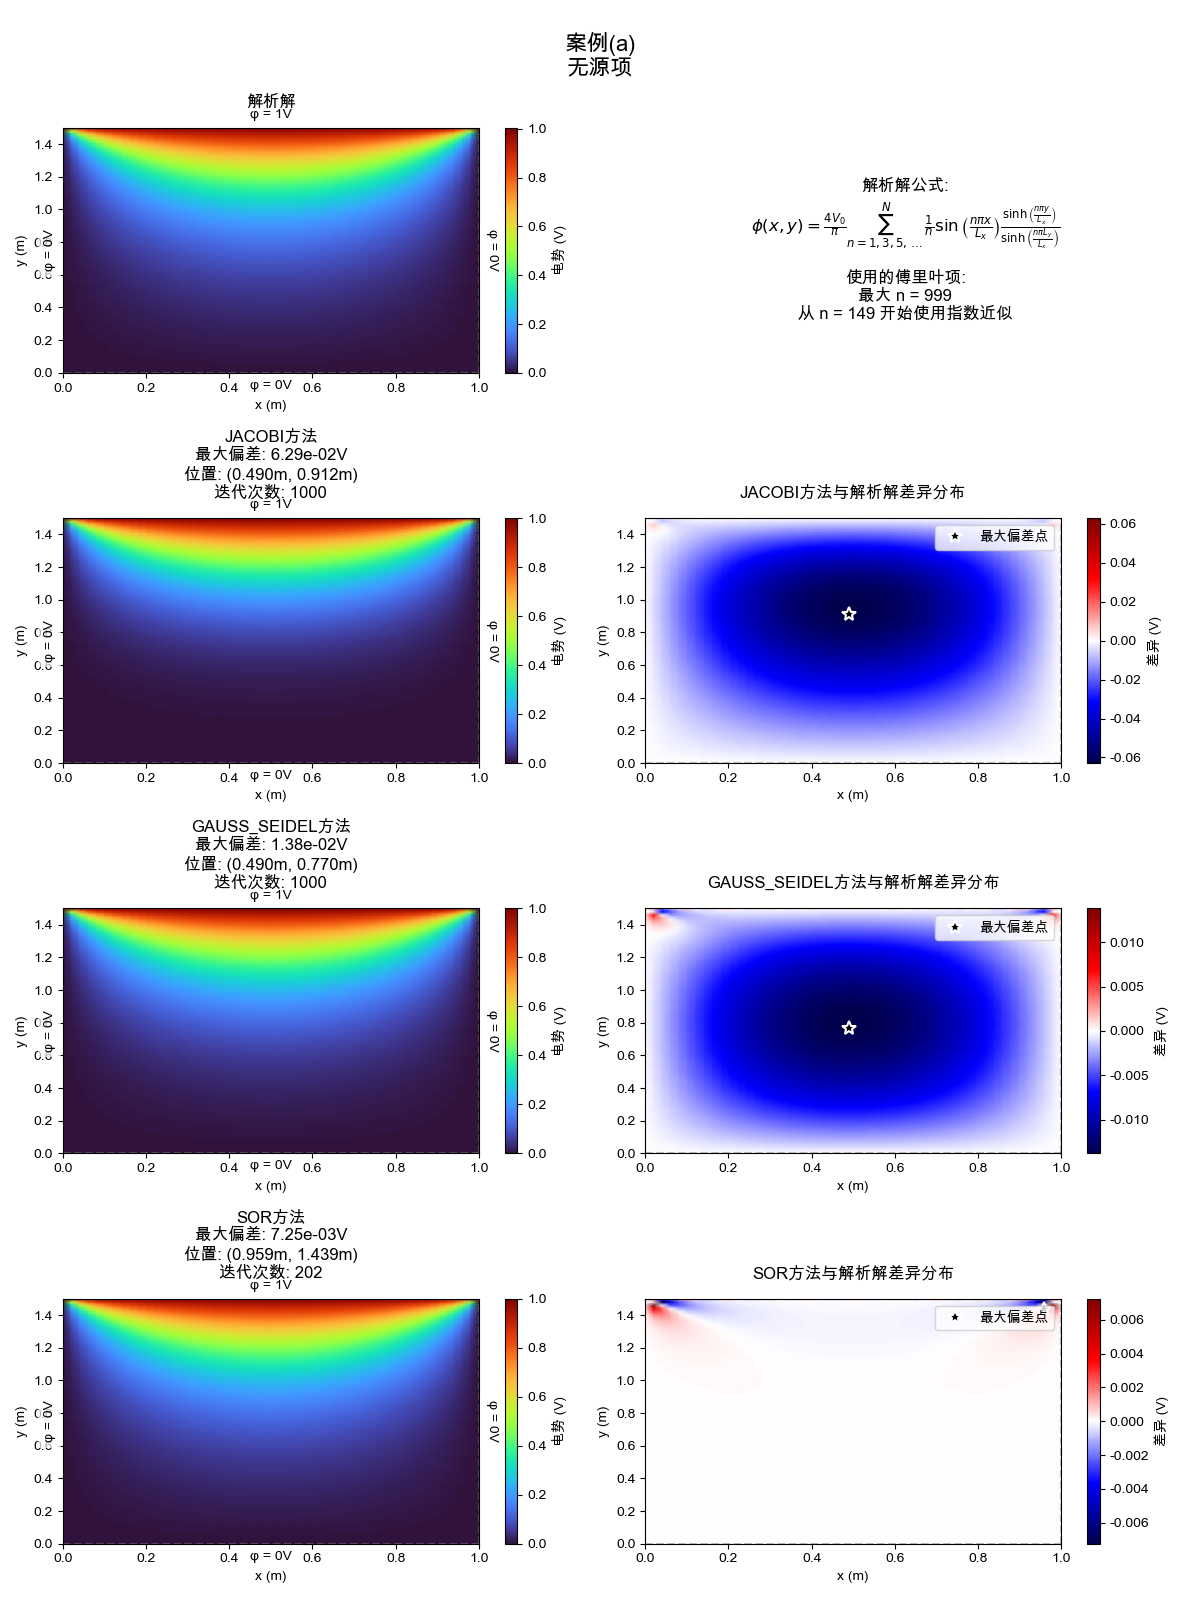
\includegraphics[width=0.9\textwidth]{Problem_1/figs/a_result.png}
    \caption{(a):计算结果及对比}
\end{figure}

\begin{figure}[H]
    \centering
    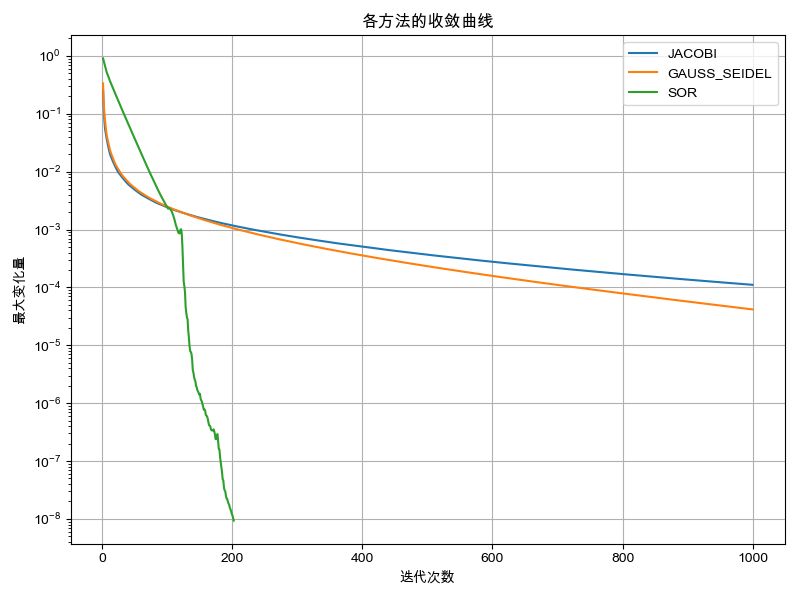
\includegraphics[width=1.0\textwidth]{Problem_1/figs/a_convergence.png}
    \caption{(a):收敛曲线对比}
\end{figure}

\subsubsection{Case (b):均匀源电荷,四边接地}
\begin{figure}[H]
    \centering
    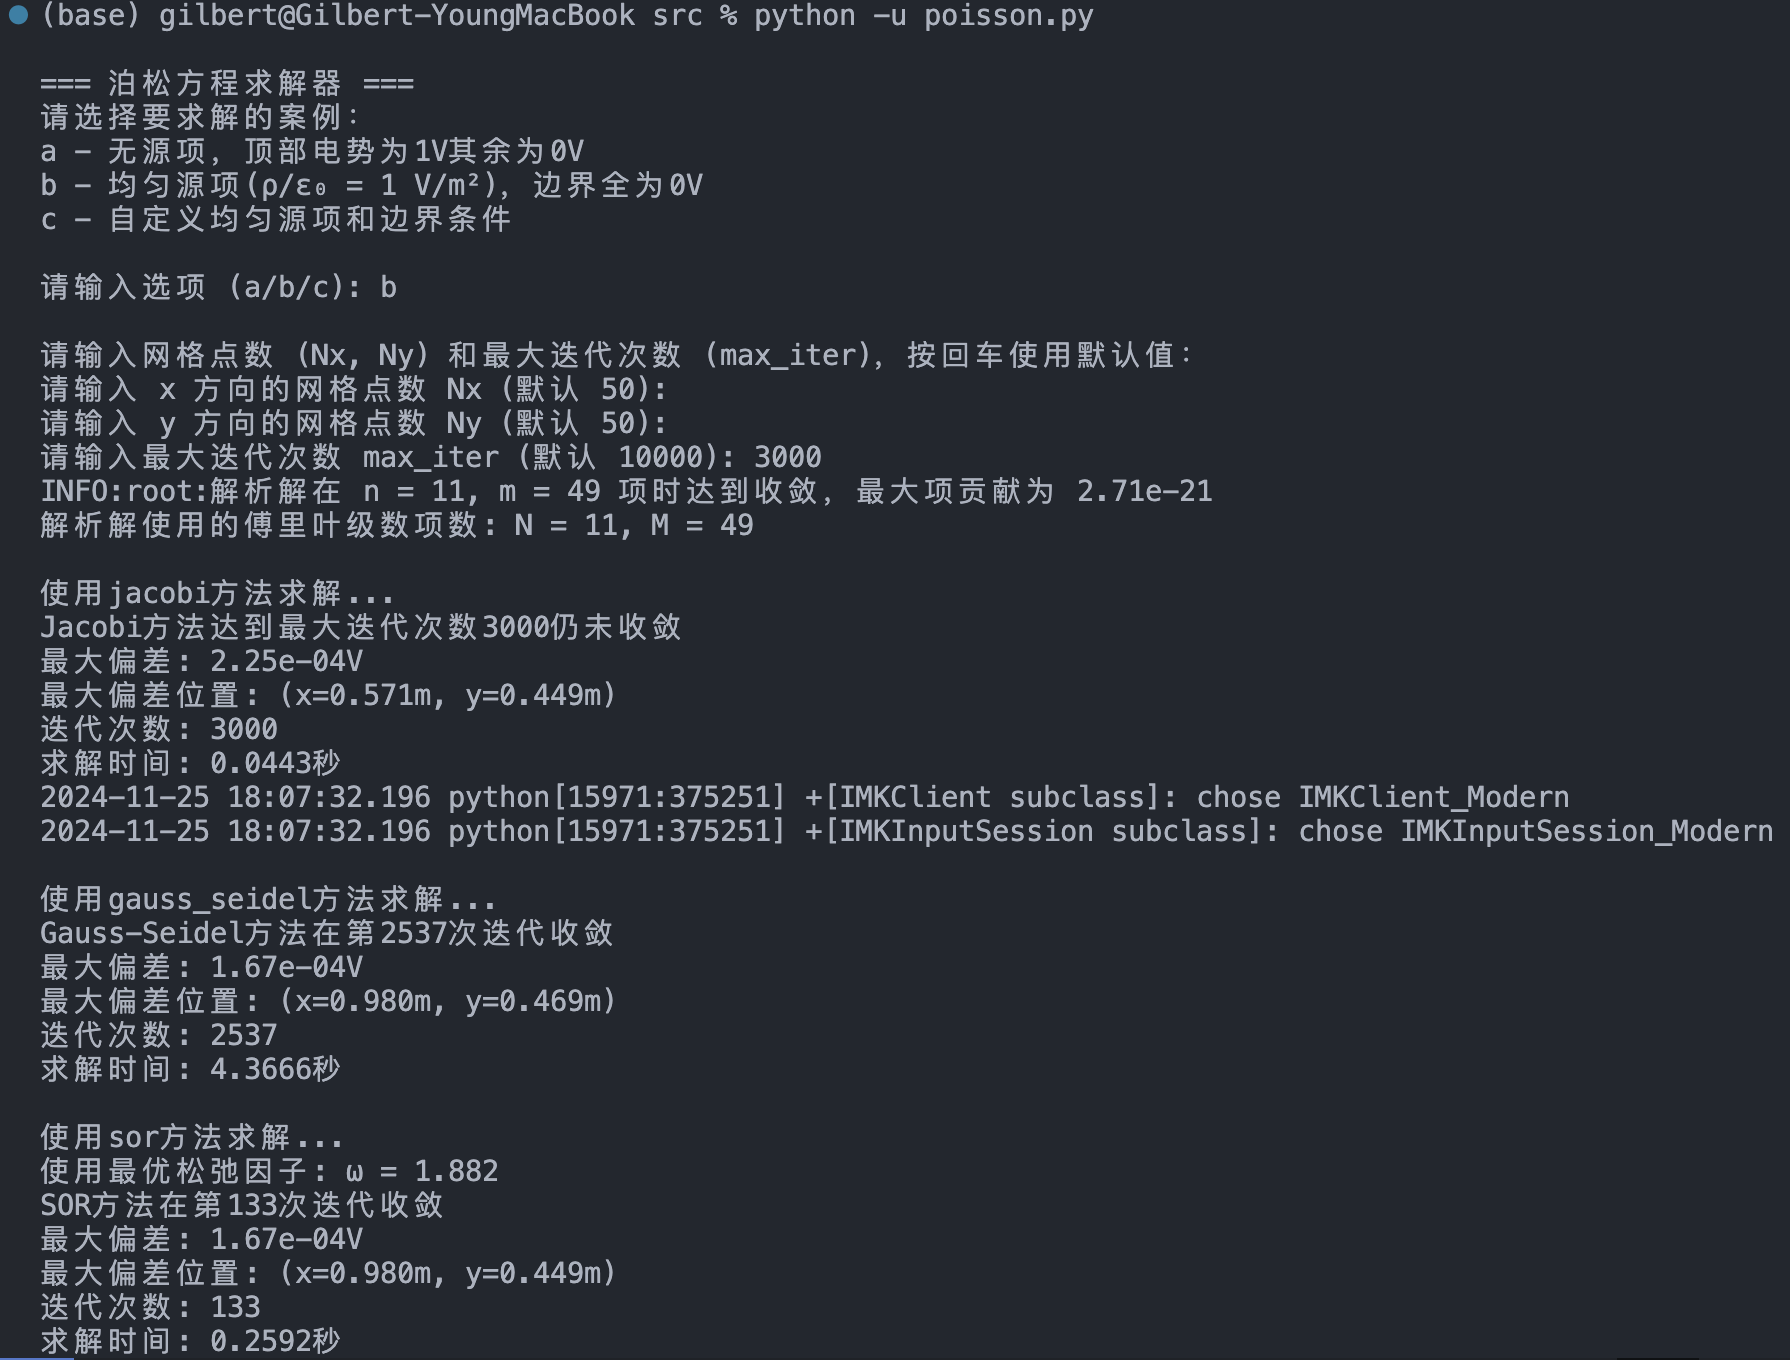
\includegraphics[width=1.0\textwidth]{Problem_1/figs/b_terminal.png}
    \caption{(b):终端输出}
\end{figure}

\begin{figure}[H]
    \centering
    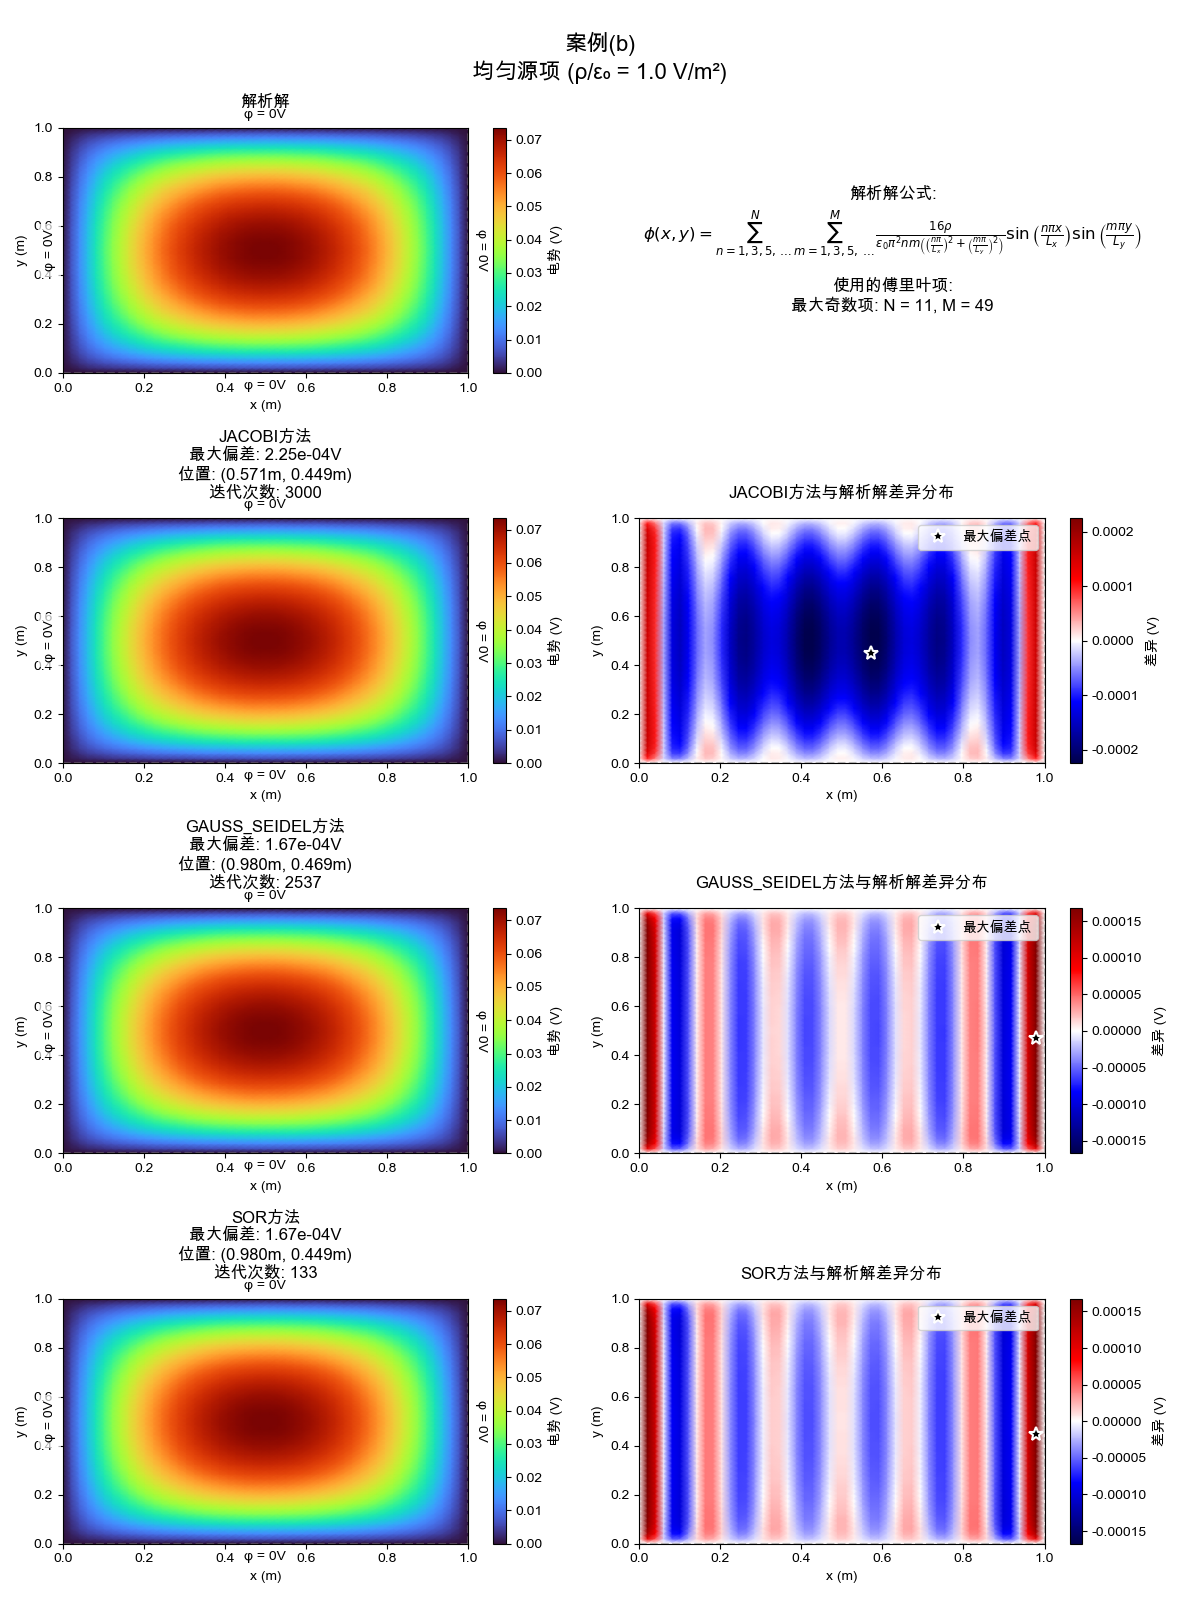
\includegraphics[width=0.9\textwidth]{Problem_1/figs/b_result.png}
    \caption{(b):计算结果及对比}
\end{figure}

\begin{figure}[H]
    \centering
    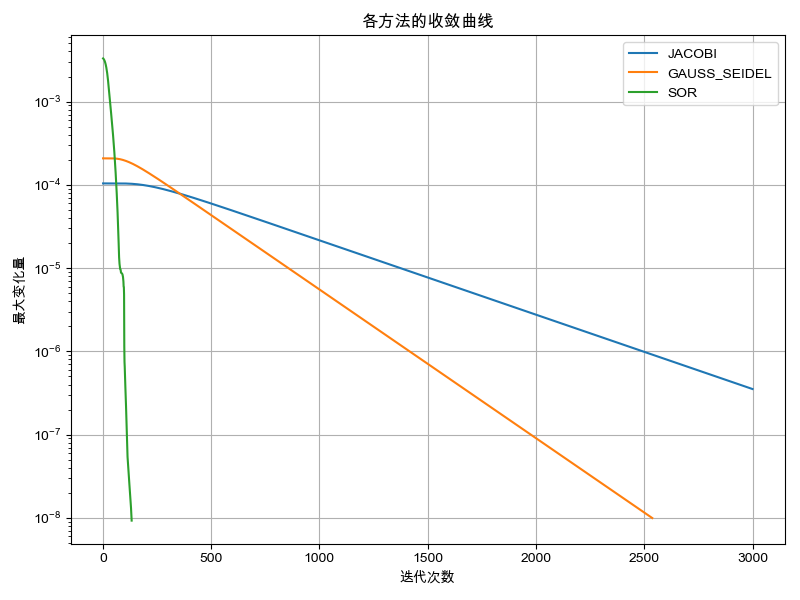
\includegraphics[width=1.0\textwidth]{Problem_1/figs/b_convergence.png}
    \caption{(b):收敛曲线对比}
\end{figure}

\subsubsection{Case (c):均匀源电荷,自定义边界}
\begin{figure}[H]
    \centering
    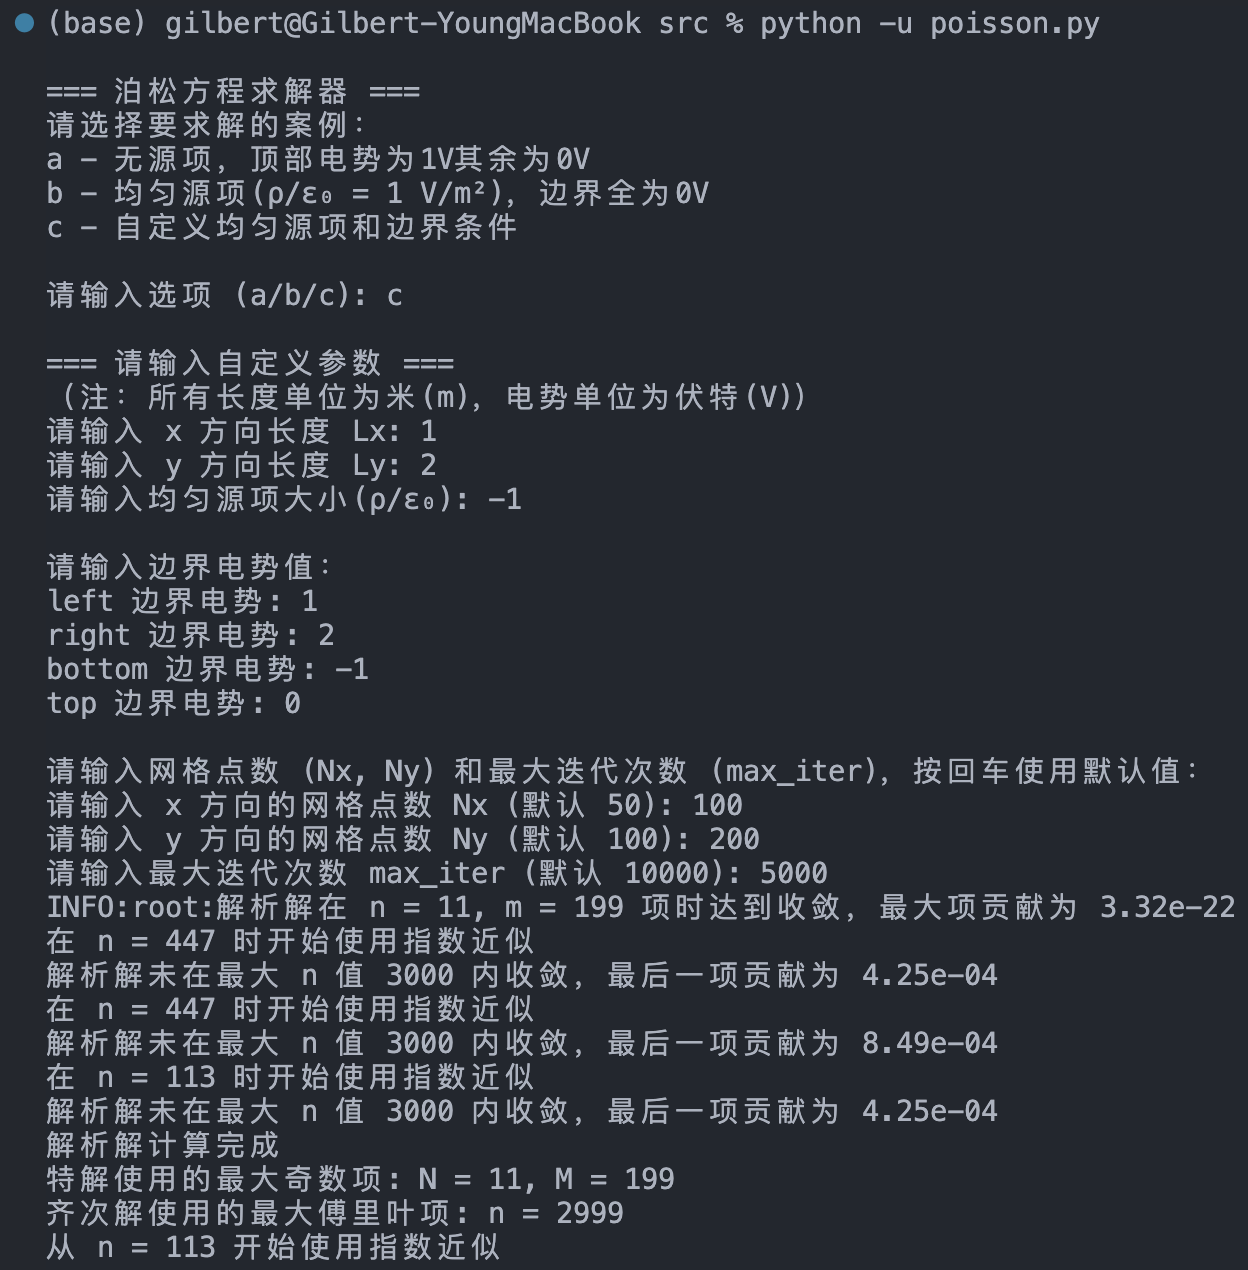
\includegraphics[width=0.5\textwidth]{Problem_1/figs/c_terminal_1.png}
    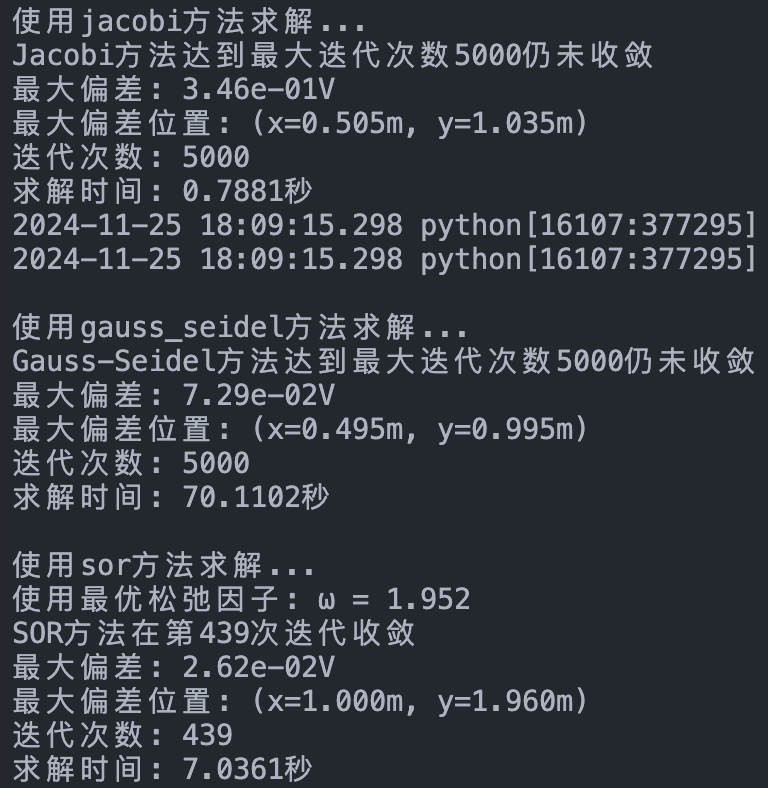
\includegraphics[width=0.5\textwidth]{Problem_1/figs/c_terminal_2.png}
    \caption{(c):终端输出}
\end{figure}

\begin{figure}[H]
    \centering
    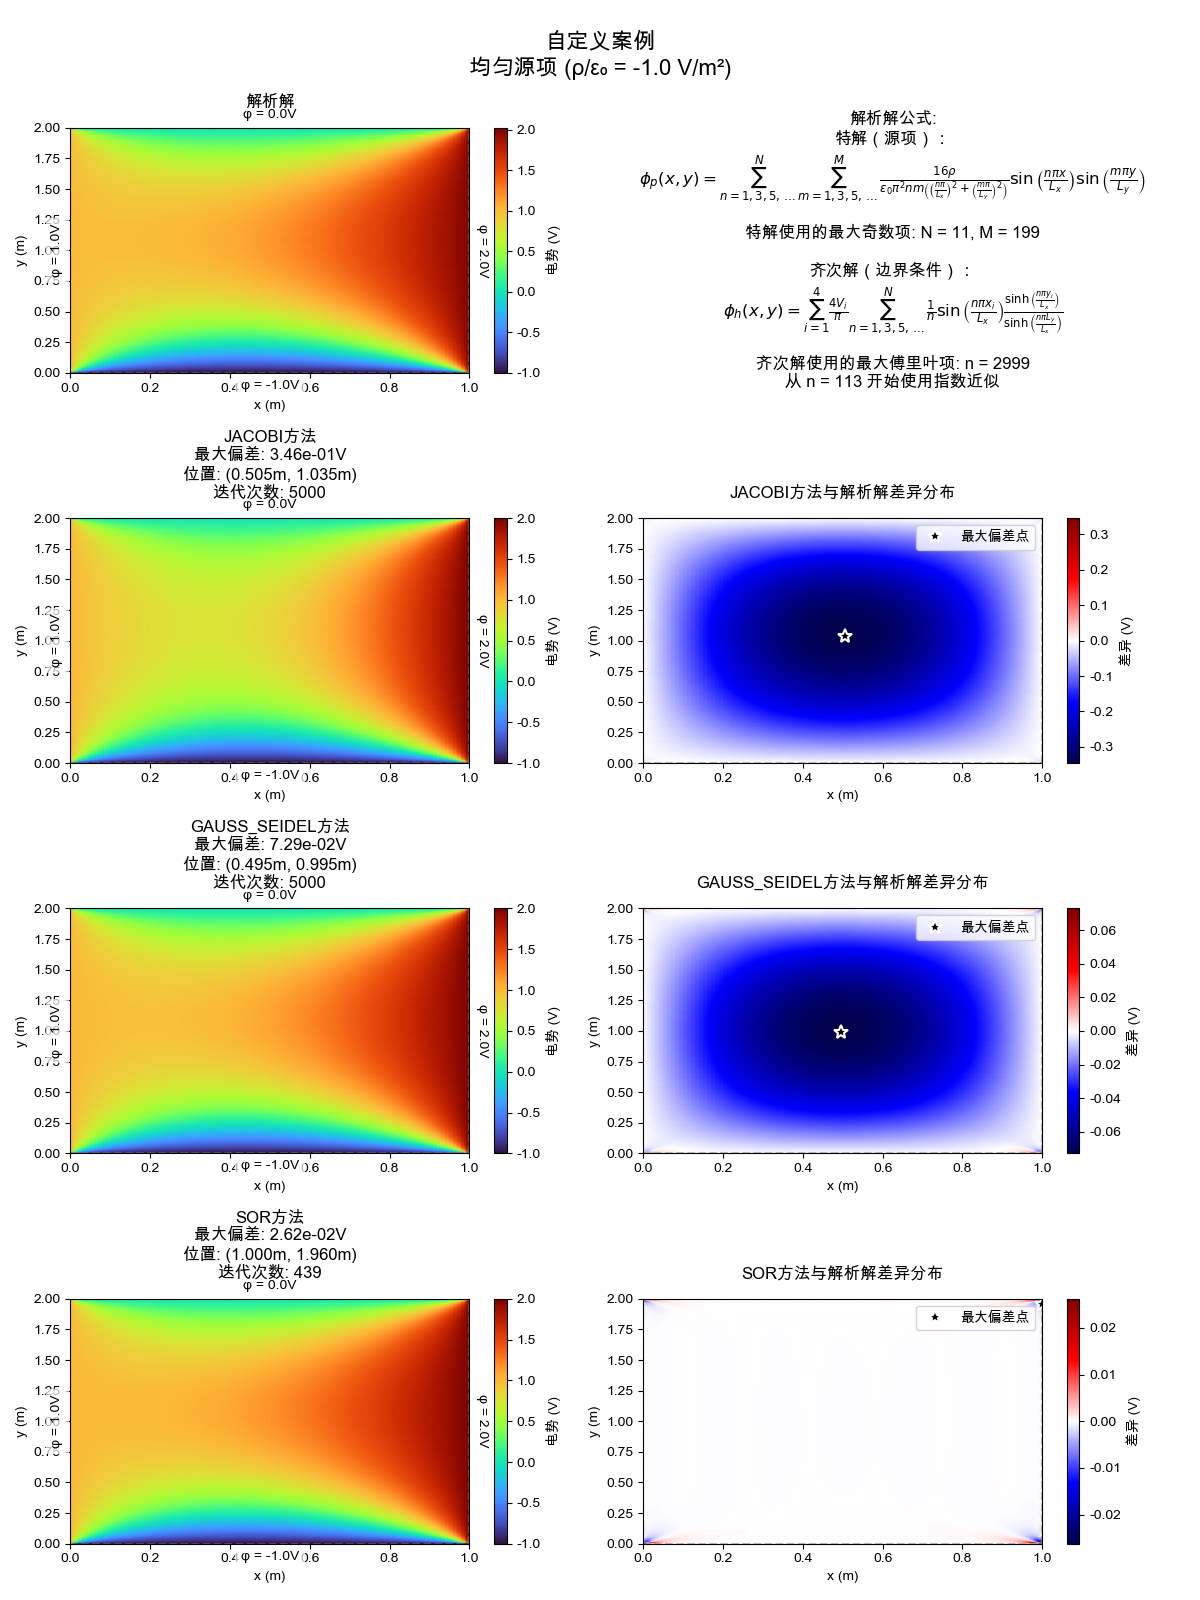
\includegraphics[width=0.9\textwidth]{Problem_1/figs/c_result.png}
    \caption{(c):计算结果及对比}
\end{figure}

\begin{figure}[H]
    \centering
    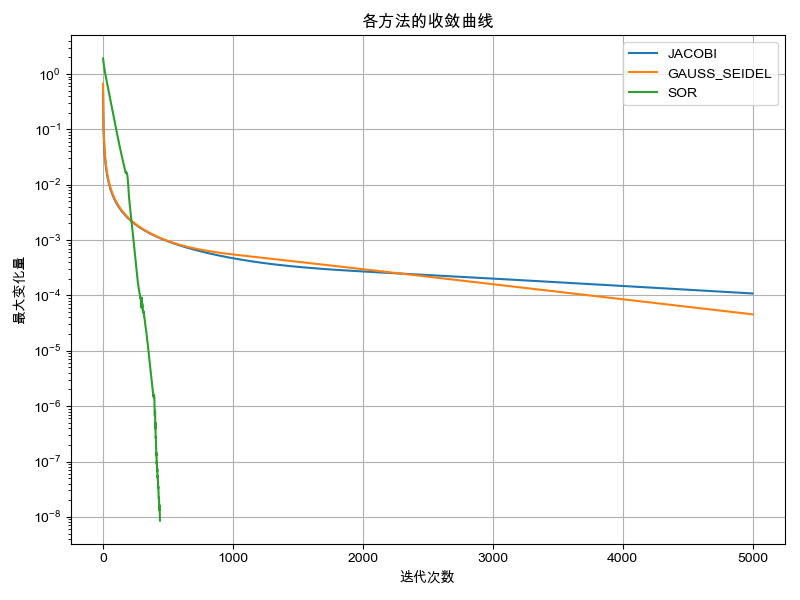
\includegraphics[width=1.0\textwidth]{Problem_1/figs/c_convergence.png}
    \caption{(c):收敛曲线对比}
\end{figure}
